\documentclass[
	% -- opções da classe memoir --
	12pt,				% tamanho da fonte
	openright,			% capítulos começam em pág ímpar (insere página vazia caso preciso)
	oneside,			% para impressão em um lado. Oposto a twoside, verso e anverso
	a4paper,			% tamanho do papel. 
	% -- opções da classe abntex2 --
	chapter=TITLE,		% títulos de capítulos convertidos em letras maiúsculas
	section=TITLE,		% títulos de seções convertidos em letras maiúsculas
	%subsection=TITLE,	% títulos de subseções convertidos em letras maiúsculas
	%subsubsection=TITLE,% títulos de subsubseções convertidos em letras maiúsculas
	% -- opções do pacote babel --
	english,			% idioma adicional para hifenização
	%french,				% idioma adicional para hifenização
	spanish,			% idioma adicional para hifenização
	brazil,				% o último idioma é o principal do documento
	]{styles/abntex2}

\usepackage{titlesec}
\usepackage[alf,abnt-etal-list=0,abnt-etal-cite=3,abnt-repeated-author-omit=no,abnt-doi=expand,abnt-emphasize=bf]{styles/abntex2cite}	% Citações padrão ABNT
\usepackage[utf8]{inputenc}
\usepackage[T1]{fontenc}
\makeatletter
\usepackage[singlelinecheck=false,justification=raggedright]{caption}
\usepackage{lastpage}
\usepackage{tabularx}
\usepackage{times}
\usepackage{graphicx}
\usepackage{styles/ttc_univali}
\usepackage{lipsum}
\usepackage{url}
\usepackage[table,xcdraw]{xcolor}
\usepackage{float}
\usepackage{accents}
\usepackage{array}
\usepackage{hyphenat}
\usepackage{multirow}
\usepackage{cancel}
\newcolumntype{C}[1]{>{\centering\arraybackslash}m{#1}}
\DeclareCaptionType{Resolucao}

%\newcolumntype{C}[1]{>{\centering\let\newline\\\arraybackslash\hspace{0pt}}m{#1}
% \usepackage[
%     % showframe=true
%     ]
% {geometry}

\title{TTC Engenharia da Computação}
\author{Modelo from Stephen Michael Apolinário}
\date{August 2022}

\hyphenation{op-tical net-works customiza-cao implementa-cao quan-do microcon-troladores} 

\begin{document}
\titleformat*{\subsubsection}{\normalfont}
\renewcommand{\arraystretch}{1.10}
\pretextual

\begin{Info}
    % Universidade
    {UNIVERSIDADE DO VALE DO ITAJAÍ}
    % Escola
    {ESCOLA DO MAR, CIÊNCIA E TECNOLOGIA}
    % Curso
    {CURSO DE ENGENHARIA DE COMPUTAÇÃO}
    % Titulo
    {relatório 03}
    % Autor
    {Stephen Michael Apolinário}
    % Cidade e Data
    {Itajaí (SC), agosto de 2022}
    % Nome da Área de concentração
    {Modelos de análise do diodo}
    % Orientador(a)
    {Walter Gontijo}
    % Coorientador(a) <Nome do Coorientador(a)>, <Titulação> %%%%%%%% Se não tiver coorientador deixe vazio
    {}
    \end{Info}
    
    % \begin{Dedicatoria}
    % Este elemento é opcional, mas caso queira fazer uma dedicatória, preencha aqui.
    % \end{Dedicatoria}
    
    % \begin{Agradecimentos}
    % Os agradecimentos são opcionais, mas este é o local adequado para isso.
    % \end{Agradecimentos}
    
    % \begin{Epigrafe}
    % A epígrafe é opcional, mas podes trazer citações, poemas, frases de impacto e citar o(s) autor(es).
    % \end{Epigrafe}
    
    \begin{Resumo}
    
    APOLINÁRIO, Stephen Michael. RELATÓRIO REFERENTE A M1 DE ELETRÔNICA BÁSICA. Itajaí, 2022. \pageref{LastPage} f. Engenharia De Computação, Escola do Mar, Ciência e Tecnologia, Universidade do Vale do Itajaí, Itajaí, 2022.
    
    
    Neste relatório, será tratado os conteúdos vistos na aula de dia 19 de agosto de 2022, na Univali Itajaí, durante a matéria de Eletrônica Básica, ministrada pelo professor Walter Antonio Gontijo, na qual foi abordado os modelos de análise de um diodo, revistando os conceitos básicos de análise, e observando o comportamento de um diodo ideal, linear e real.
    
    Palavras-chave: Díodo ideal, Diodo Real, Diodo Linear.
    
    \end{Resumo} \clearpage
% ---
% inserir lista de ilustrações
% ---
\pdfbookmark[0]{\listfigurename}{lof}
\listoffigures*
\cleardoublepage
% ---

% ---
% inserir lista de tabelas
% ---
% \pdfbookmark[0]{\listtablename}{lot}
% \listoftables*
% \cleardoublepage
% ---

% ---
% inserir lista de quadros
% ---
\pdfbookmark[0]{\listofquadrosname}{loq}
\listofquadros*
\cleardoublepage
% ---

% ---
% inserir lista de abreviaturas e siglas
% ---
\begin{siglas}
    \item[PCD] Pessoa com deficiência
    \item[PWD] Person with disability
    \item[MOVI] Museu Oceanográfico Univali
    \item[MVP]  Minimum Viable Product
    \item[TIC] Trabalho de iniciação cientifica 

\end{siglas}
% ---

% ---
% inserir lista de símbolos
% ---
%\begin{simbolos}
%  \item[$ \Gamma $] Letra grega Gama
%  \item[$ \Lambda $] Lambda
%  \item[$ \zeta $] Letra grega minúscula zeta
% \item[$ \in $] Pertence
%\end{simbolos}
% ---

% ---
% inserir o sumario
% ---
\pdfbookmark[0]{\contentsname}{toc}
\tableofcontents*
\cleardoublepage
% --- \clearpage

\textual % Indica inicio dos elementos textuais
\pagestyle{simple} % remove o cabeçalho
\chapter{OBJETIVOS}

Os objetivos deste relatório possuem obter o conhecimento dos seguintes tópicos:

\begin{enumerate}
    \item Revisar análise de circuito.
    \item Modelos de análise de circuito.
    \item Comportamento de diodo em diferentes modelos de análise.
\end{enumerate} \clearpage
\chapter{INTRODUÇÃO}

Os diodos abordados nas aulas referenciadas neste relatório, são componentes eletrônicos que possuem a função de permitir a passagem de corrente elétrica em apenas uma direção. Sendo assim, os diodos são componentes semicondutores que possuem uma característica de polarização, ou seja, a passagem de corrente elétrica só ocorre quando o diodo é polarizado. Estes componentes são muito importantes para a eletrônica, pois através deles é possível criar circuitos mais complexos com a utilização de outros componentes eletrônicos. \clearpage
\chapter{DESENVOLVIMENTO}

\section{Retificador de meia onda}

\subsection{Circuito A}

\begin{figure}[H]
    \centering
    \fbox{
        \parbox{0.975\textwidth}{
            \centering
            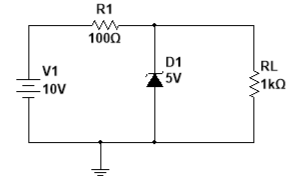
\includegraphics[width=0.975\textwidth]{images/imagem_slide_01.png}
        }}
    \caption{Retificador - Meia Onda}
    \vspace{-0.3cm}
    \label{fig:ImagemSlide01}
\end{figure}

\begin{figure}[H]
    \centering
    \fbox{
        \parbox{0.975\textwidth}{
            \centering
            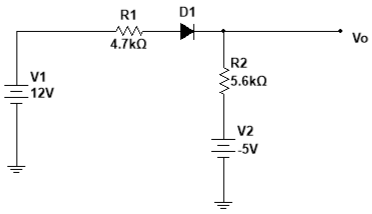
\includegraphics[]{images/simulacoes/Circuito01.png}
        }}
    \caption{Simulação: Circuito retificador de meia onda}
    \vspace{-0.3cm}
    \label{fig:SimulacaoCircuito01}
\end{figure}

\noindent
\textbf{Resolução}

\begin{Resolucao}[H]
    \fbox{
        \parbox{0.975\textwidth}{
            \vspace{0.40cm}
            \centering
            Utilizando um diodo simplificado com queda de tensão de 0.7V\dots

            \[Vin = 5v\]
            \[\textnormal{Vpk na saída} = 5V - 0.7V = \textcolor{red}{4.3V}\]
            \[\textnormal{VDC na saída} = \frac{4.3V}{\pi} = \textcolor{red}{1.368V}\]

            \[\textnormal{Tensão da fonte} = \frac{5}{\sqrt[2]{2}} \simeq \textcolor{red}{3.53V}\]
        }
    }
    \captionof{Resolucao}{Resolução: Circuito retificador de meia onda}
    \label{res:CircuitoExercicio}
\end{Resolucao}

\begin{figure}[H]
    \centering
    \fbox{
        \parbox{0.975\textwidth}{
            \centering
            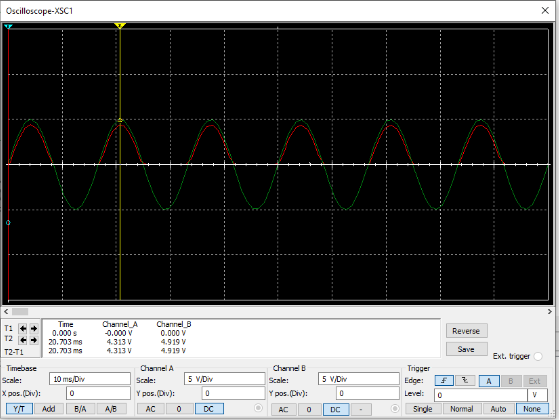
\includegraphics[width=0.975\textwidth]{images/simulacoes/osciloscopio_circuito01.png}
        }}
    \caption{Osciloscópio: Circuito retificador de meia onda}
    \vspace{-0.3cm}
    \label{fig:OsciloscopioCircuito01}
\end{figure}

\begin{figure}[H]
    \centering
    \fbox{
        \parbox{0.975\textwidth}{
            \centering
            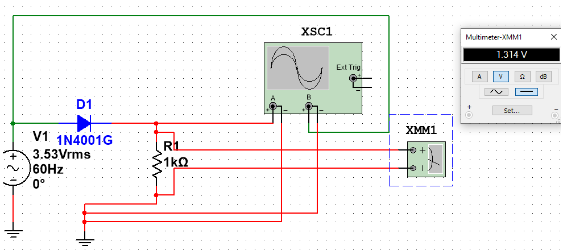
\includegraphics[]{images/simulacoes/Circuito01Multimetro.png}
        }}
    \caption{Simulação: Multímetro circuito retificador de meia onda}
    \vspace{-0.3cm}
    \label{fig:SimulacaoCircuito01Multimetro}
\end{figure}

Através das imagens acima, é possível comparar nossos resultados com os valores obtidos por cálculos, mas por facilidade, iremos comparar utilizando a tabela \ref{tab:Comparacao1Circuito}

\begin{quadro}[H]
    \centering
    \caption{Comparação entre os resultados obtidos por simulação e os resultados obtidos por cálculo do circuito 01}
    \begin{tabular}{|C{0.19\textwidth}|C{0.24\textwidth}|C{0.24\textwidth}|C{0.24\textwidth}|C{0.24\textwidth}|}
        \hline
        \rowcolor[HTML]{C0C0C0}
        \textbf{Modelo\textbackslash{}Variáveis} & \textbf{Tensão Pico de entrada} & \textbf{Tensão Pico de saída} & \textbf{Tensão Média de saída} \\
        \hline
        Calculado & 5V & 4.3V & 1.368V \\
        \hline
        Simulado & 4.919V & 4.313V & 1.314V \\
        \hline
    \end{tabular}
    \vspace{-0.6cm}
    \label{tab:Comparacao1Circuito}
\end{quadro}

\subsection{Circuito B}

Calcule o seguinte circuito, considerando o diodo simplificado com queda de tensão de 0.7V:

\noindent
\textbf{Circuito B}

\begin{Resolucao}[H]
    \fbox{
        \parbox{0.975\textwidth}{
            \vspace{0.40cm}
            \centering
            \[Vin = 100V\]
            \[\textnormal{Vpk na saída} = 100V - 0.7V = \textcolor{red}{99.3V}\]
            \[\textnormal{VDC na saída} = \frac{99.3V}{\pi} = \textcolor{red}{31.5V}\]	

            \[\textnormal{Tensão da fonte} = \frac{100}{\sqrt[2]{2}} \simeq \textcolor{red}{70.71V}\]
        }
    }
    \captionof*{Resolucao}{Resolução: Circuito Exercício B}
    \label{res:CircuitoExercicioB}
\end{Resolucao}

\begin{figure}[H]
    \centering
    \fbox{
        \parbox{0.975\textwidth}{
            \centering
            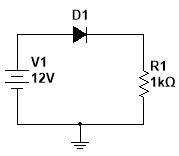
\includegraphics[]{images/simulacoes/Circuito02.png}
        }}
    \caption{Simulação: Multímetro circuito retificador de meia onda}
    \vspace{-0.3cm}
    \label{fig:SimulacaoCircuito02}
\end{figure}

\begin{figure}[H]
    \centering
    \fbox{
        \parbox{0.975\textwidth}{
            \centering
            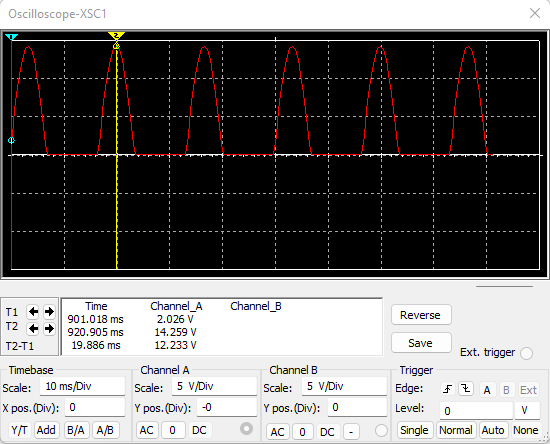
\includegraphics[width=0.975\textwidth]{images/simulacoes/osciloscopio_circuito02.png}
        }}
    \caption{Osciloscópio: Circuito retificador de meia onda B}
    \vspace{-0.3cm}
    \label{fig:OsciloscopioCircuito02}
\end{figure}

Através da imagem \ref{fig:SimulacaoCircuito02}, é possível observar que a tensão média na saída é de 1.314V. E a imagem \ref{fig:OsciloscopioCircuito02} mostra que a tensão pico na saída é de 99.227V.

Com a tabela \ref{tab:Comparacao2Circuito} podemos comparar os resultados obtidos por simulação com os resultados obtidos por cálculo, na qual comprovam que os cálculos estavam corretos, com uma pequena diferença devido a aproximação.

\begin{quadro}[H]
    \centering
    \caption{Comparação entre os resultados obtidos por simulação e os resultados obtidos por cálculo do circuito 02}
    \begin{tabular}{|C{0.19\textwidth}|C{0.24\textwidth}|C{0.24\textwidth}|C{0.24\textwidth}|C{0.24\textwidth}|}
        \hline
        \rowcolor[HTML]{C0C0C0}
        \textbf{Modelo\textbackslash{}Variáveis} & \textbf{Tensão Pico de entrada} & \textbf{Tensão Pico de saída} & \textbf{Tensão Média de saída} \\
        \hline
        Calculado & 100V & 99.3V & 31.68V \\
        \hline
        Simulado & 99.227V & 98.468V & 31.615V \\
        \hline
    \end{tabular}
    \vspace{-0.6cm}
    \label{tab:Comparacao2Circuito}
\end{quadro}

\subsection{Circuito C}

Calcule o seguinte circuito:

\begin{figure}[H]
    \centering
    \fbox{
        \parbox{0.975\textwidth}{
            \centering
            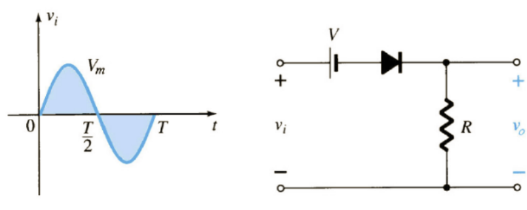
\includegraphics[width=0.975\textwidth]{images/imagem_slide_02.png}
        }}
    \caption{Retificador - Meia Onda}
    \vspace{-0.3cm}
    \label{fig:ImagemSlide02}
\end{figure}

\noindent
\textbf{Circuito C}

\begin{Resolucao}[H]
    \fbox{
        \parbox{0.975\textwidth}{
            \vspace{0.40cm}
            \centering
            \[Vin = 170V\]
            \[n = \frac{1}{2} 0.5V\]
            \[\textnormal{Vpk de entrada no secundário:} Vin * n = 170 * 0.5V = \textcolor{red}{85V}\]
            \[\textnormal{Vpk na saída} = 85V - 0.7V = \textcolor{red}{84.3}\]
            \[\textnormal{VDC na entrada} = \frac{170}{\sqrt[2]{2}} \simeq \textcolor{red}{120.21V}\]
            \[\textnormal{VDC na saída} = \frac{84.3}{\pi} \simeq \textcolor{red}{26.8V}\]
        }
    }
    \captionof*{Resolucao}{Resolução: Circuito Exercício C}
    \label{res:CircuitoExercicioC}
\end{Resolucao}

\begin{figure}[H]
    \centering
    \fbox{
        \parbox{0.975\textwidth}{
            \centering
            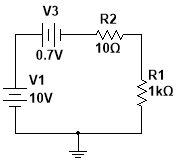
\includegraphics[]{images/simulacoes/Circuito03.png}
        }}
    \caption{Simulação: Circuito meia onda C}
    \vspace{-0.3cm}
    \label{fig:SimulacaoCircuito03}
\end{figure}

\begin{figure}[H]
    \centering
    \fbox{
        \parbox{0.975\textwidth}{
            \centering
            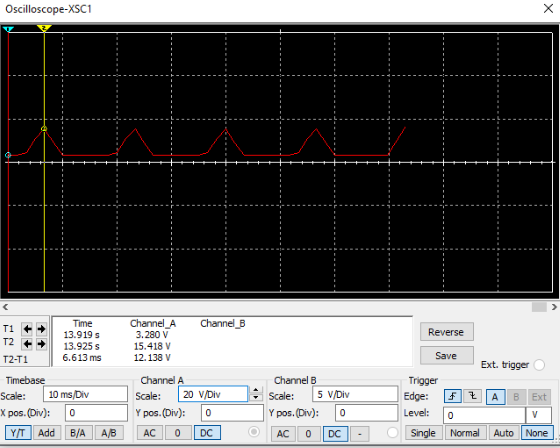
\includegraphics[width=0.975\textwidth]{images/simulacoes/osciloscopio_circuito03.png}
        }}
    \caption{Osciloscópio: Circuito retificador de meia onda C}
    \vspace{-0.3cm}
    \label{fig:OsciloscopioCircuito02}
\end{figure}

Com a tabela \ref{tab:Comparacao3Circuito} podemos comparar os resultados obtidos por simulação com os resultados obtidos por cálculo, na qual comprovam que os cálculos estavam corretos, com uma pequena diferença devido a aproximação.

\begin{quadro}[H]
    \centering
    \caption{Comparação entre os resultados obtidos por simulação e os resultados obtidos por cálculo do circuito 03}
    \begin{tabular}{|C{0.19\textwidth}|C{0.18\textwidth}|C{0.18\textwidth}|C{0.18\textwidth}|C{0.18\textwidth}|}
        \hline
        \rowcolor[HTML]{C0C0C0}
        \textbf{Modelo\textbackslash{}Variáveis} & \textbf{Tensão Pico de entrada 1$\circ$} & \textbf{Tensão Pico de entrada 2$\circ$} & \textbf{Tensão de pico de saída 2$\circ$} & \textbf{Tensão média (Avg) de saída 2$\circ$} \\
        \hline
        Calculado & 170.00V & 85.000V & 84.300V & 26.830V \\
        \hline
        Simulado & 166.53V & 82.516V & 82.516V & 26.767V \\
        \hline
    \end{tabular}
    \vspace{-0.6cm}
    \label{tab:Comparacao3Circuito}
\end{quadro}

\subsection{Circuito D}

\begin{figure}[H]
    \centering
    \fbox{
        \parbox{0.975\textwidth}{
            \centering
            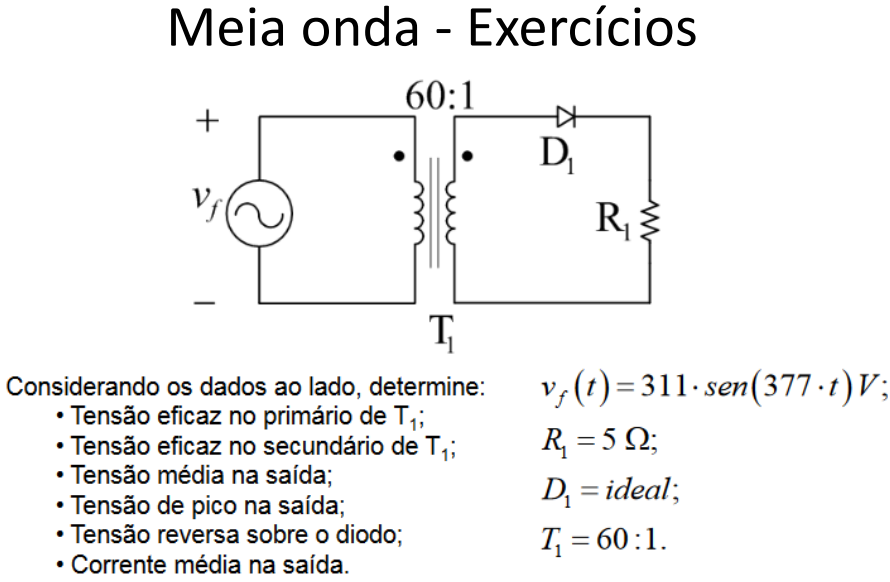
\includegraphics[width=0.975\textwidth]{images/imagem_slide_03.png}
        }}
    \caption{Retificador - Meia Onda D}
    \vspace{-0.3cm}
    \label{fig:ImagemSlide03}
\end{figure}

\begin{Resolucao}[H]
    \fbox{
        \parbox{0.975\textwidth}{
            \vspace{0.40cm}
            \centering
            \[Vp = 311V\]
            \[n = \frac{1}{60}\]
            \[Vpico = Vp * n \]

            \[\textnormal{Tensão eficaz no primário de T1: } \frac{311}{\sqrt[2]{2}} = \textcolor{red}{220V}\]
            \[\textnormal{Tensão eficaz no secundário de T1: } \frac{Eficaz1}{Fator} \rightarrow \frac{220}{60} = \textcolor{red}{3.66V} \]
            \[\textnormal{Tensão de pico de entrada no secundário: } Vpico \simeq \textcolor{red}{5.18V}\]
            \[\textnormal{Tensão média na saída: } \frac{Vpico - (0.7 * 1)}{\pi} \simeq \textcolor{red}{1.43V}\]
            \[\textnormal{Tensão de pico na saída: } Vpico - 0.7 = \textcolor{red}{4.483V}\]
            \[\textnormal{Tensão reversa sobre o diodo: } \textcolor{red}{-5.18V}\]
            \[\textnormal{Corrente média na saída: }  \frac{TensaoMédia}{Ressistencia} \rightarrow \frac{1.43}{5} \simeq \textcolor{red}{0.286A}\]
        }
    }
    \captionof*{Resolucao}{Resolução: Circuito Exercício D}
    \label{res:CircuitoExercicioD}
\end{Resolucao}

\begin{figure}[H]
    \centering
    \fbox{
        \parbox{0.975\textwidth}{
            \centering
            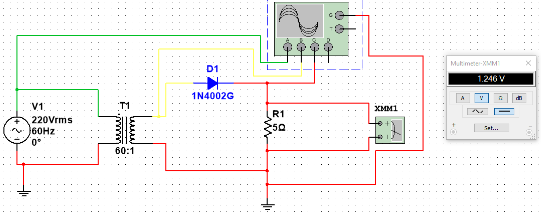
\includegraphics[]{images/simulacoes/Circuito04.png}
        }}
    \caption{Simulação: Circuito meia onda D}
    \vspace{-0.3cm}
    \label{fig:SimulacaoCircuito04}
\end{figure}

\begin{figure}[H]
    \centering
    \fbox{
        \parbox{0.975\textwidth}{
            \centering
            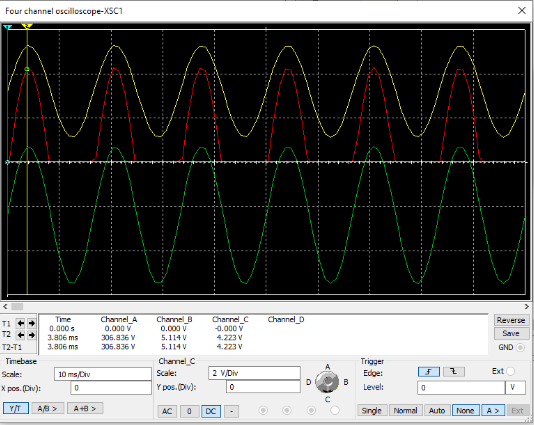
\includegraphics[width=0.975\textwidth]{images/simulacoes/osciloscopio_circuito04.png}
        }}
    \caption{Osciloscópio: Circuito retificador de meia onda D}
    \vspace{-0.3cm}
    \label{fig:OsciloscopioCircuito04}
\end{figure}

Através da imagem \ref{fig:OsciloscopioCircuito04}, é possível observar que a linha em verde representa a onda do sinal de entrada primário, já a linha amarela é o sinal de entrada transformado, ou seja, o sinal secundário. Já a linha em vermelho, representa o sinal de saída do circuito.

Com a tabela \ref{tab:Comparacao4Circuito} podemos comparar os resultados obtidos por simulação com os resultados obtidos por cálculo, na qual comprovam que os cálculos estavam corretos, com uma pequena diferença devido a aproximação.

\begin{quadro}[H]
    \centering
    \caption{Comparação entre os resultados obtidos por simulação e os resultados obtidos por cálculo do circuito 02}
    \begin{tabular}{|C{0.19\textwidth}|C{0.18\textwidth}|C{0.18\textwidth}|C{0.18\textwidth}|C{0.18\textwidth}|}
        \hline
        \rowcolor[HTML]{C0C0C0}
        \textbf{Modelo\textbackslash{}Variáveis} & \textbf{Tensão Pico primária} & \textbf{Tensão Pico secundária} & \textbf{Tensão pico de saída} & \textbf{Tensão pico média}\\
        \hline
        Calculado & 311V & 5.18V & 4.48V & 1.426V \\
        \hline
        Simulado & 306.256V & 5.104V & 4.28V & 1.426V \\
        \hline
    \end{tabular}
    \vspace{-0.6cm}
    \label{tab:Comparacao4Circuito}
\end{quadro}

\section{Circuito retificador de onda completa}

\subsection{Circuito A}

\begin{figure}[H]
    \centering
    \fbox{
        \parbox{0.975\textwidth}{
            \centering
            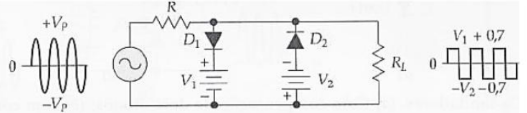
\includegraphics[width=0.975\textwidth]{images/imagem_slide_04.png}
        }}
    \caption{Retificador - Onda Completa A}
    \vspace{-0.3cm}
    \label{fig:ImagemSlide04}
\end{figure}

\noindent
\textbf{Circuito A}

\begin{Resolucao}[H]
    \fbox{
        \parbox{0.975\textwidth}{
            \vspace{0.40cm}
            \centering
            \[Vf = 100V\]
            \[n = \frac{1}{2}\]
            \[\textnormal{Tensão de pico de entrada no 2$\circ$} = Vp * 100 * \frac{1}{2} = \textcolor{red}{50V}\]
            \[\textnormal{Tensão de pico na saída} = 50V * 0.5 - 0.7V = \textcolor{red}{24.3V}\]
            \[\textnormal{Tensão média ou DC de saída} = \frac{2Vp}{\pi} = \textcolor{red}{15.46V}\]
        }
    }
    \captionof*{Resolucao}{Resolução: Circuito Exercício A}
    \label{res:CircuitoExercicioOndaCompletaA}
\end{Resolucao}

\begin{figure}[H]
    \centering
    \fbox{
        \parbox{0.975\textwidth}{
            \centering
            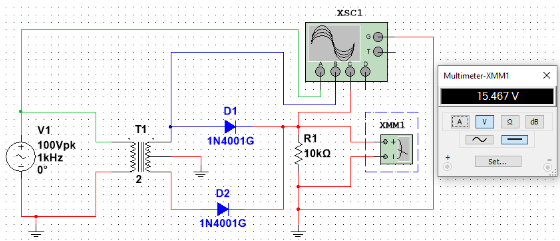
\includegraphics[]{images/simulacoes/Circuito05.png}
        }}
    \caption{Simulação: Circuito onda completa A}
    \vspace{-0.3cm}
    \label{fig:SimulacaoCircuito05OndaCompleta}
\end{figure}

\begin{figure}[H]
    \centering
    \fbox{
        \parbox{0.975\textwidth}{
            \centering
            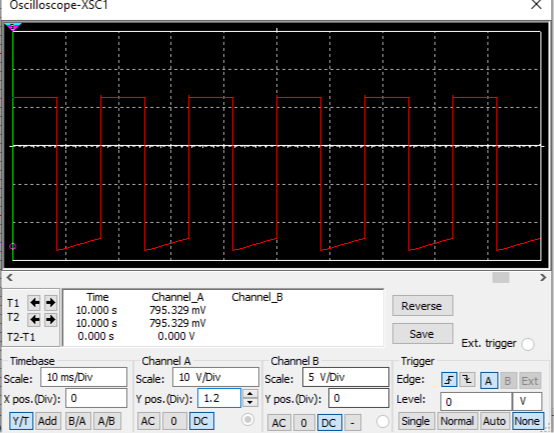
\includegraphics[width=0.975\textwidth]{images/simulacoes/osciloscopio_circuito05.png}
        }}
    \caption{Osciloscópio: Circuito retificador de onda completa A}
    \vspace{-0.3cm}
    \label{fig:OsciloscopioCircuito05}
\end{figure}

Através da imagem \ref{fig:OsciloscopioCircuito05}, podemos observar que as ondas em verdes são a de tensão de entrada, na qual a mesma atinge aproximadamente 100v. A linha azul representa a tensão de entrada na secundária, de aproximadamente 50V, na qual está sendo dividida entre a parte de baixo e a de cima do circuito, sendo aproximadamente 25V para o diodo D1 e 25V para o diodo D2. A tensão de saída obtida é a tensão sobre o resistor, e o sinal de saída tem o dobro da frequência.

Com a tabela \ref{tab:Comparacao5Circuito} podemos comparar os resultados obtidos por simulação com os resultados obtidos por cálculo, na qual comprovam que os cálculos estavam corretos, com uma pequena diferença devido a aproximação.

\begin{quadro}[H]
    \centering
    \caption{Comparação entre os resultados obtidos por simulação e os resultados obtidos por cálculo do circuito A}
    \begin{tabular}{|C{0.19\textwidth}|C{0.18\textwidth}|C{0.18\textwidth}|C{0.18\textwidth}|C{0.18\textwidth}|}
        \hline
        \rowcolor[HTML]{C0C0C0}
        \textbf{Modelo\textbackslash{}Variáveis} & \textbf{Tensão Pico primária} & \textbf{Tensão Pico secundária} & \textbf{Tensão pico de saída} & \textbf{Tensão pico média}\\
        \hline
        Calculado & 100V & 50V & 24.38V & 15.46V \\
        \hline
        Simulado & 99.309V & 49.63V & 24.236V & 15.46V \\
        \hline
    \end{tabular}
    \vspace{-0.6cm}
    \label{tab:Comparacao5Circuito}
\end{quadro}

\subsection{Circuito B}

\begin{figure}[H]
    \centering
    \fbox{
        \parbox{0.975\textwidth}{
            \centering
            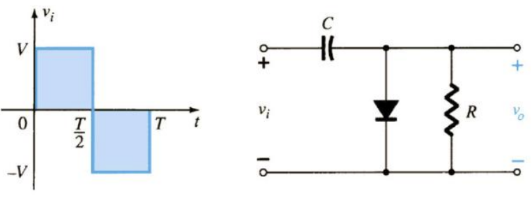
\includegraphics[width=0.975\textwidth]{images/imagem_slide_05.png}
        }}
    \caption{Retificador - Onda Completa B}
    \vspace{-0.3cm}
    \label{fig:ImagemSlide05}
\end{figure}


\noindent
\textbf{Circuito B}

\begin{Resolucao}[H]
    \fbox{
        \parbox{0.975\textwidth}{
            \vspace{0.40cm}
            \centering
            \[Vp = \textcolor{red}{311V}\]
            \[n = \frac{100}{500} = \textcolor{red}{0.2}\]
            \[Vpico = Vp * n \]

            \[\textnormal{Tensão eficaz no primário de T1: } \frac{311}{\sqrt[2]{2}} = \textcolor{red}{220V}\]
            \[\textnormal{Tensão eficaz no secundário de T1: } \frac{Eficaz1}{Fator} \rightarrow 220 * 0.2 = \textcolor{red}{44V} \]
            \[\textnormal{Tensão de pico de entrada no secundário: } Vpico = 311 * 0.2 \simeq \textcolor{red}{62.2V}\]
            \[\textnormal{Tensão média na saída: }  \frac{2 * Vpico(saida)}{\pi} \simeq \textcolor{red}{19.35V}\]
            \[\textnormal{Tensão de pico na saída: } \frac{Vpico}{2} - 0.7 = \textcolor{red}{30.4V}\]
            \[\textnormal{Tensão reversa sobre o diodo: } -(62.2V - 0,7V)  \textcolor{red}{-61.5V}\]
            \[\textnormal{Corrente média na saída: }  \frac{TensaoMédia}{Ressistencia} \rightarrow \frac{19.35}{5} \simeq \textcolor{red}{3.87A}\]
        }
    }
    \captionof*{Resolucao}{Resolução: Circuito Exercício B}
    \label{res:CircuitoExercicioOndaCompletaB}
\end{Resolucao}

\begin{figure}[H]
    \centering
    \fbox{
        \parbox{0.975\textwidth}{
            \centering
            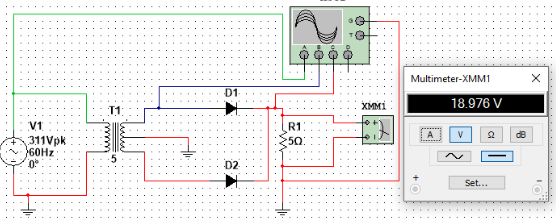
\includegraphics[]{images/simulacoes/Circuito06.png}
        }}
    \caption{Simulação: Circuito onda completa B}
    \vspace{-0.3cm}
    \label{fig:SimulacaoCircuito06OndaCompleta}
\end{figure}

\begin{figure}[H]
    \centering
    \fbox{
        \parbox{0.975\textwidth}{
            \centering
            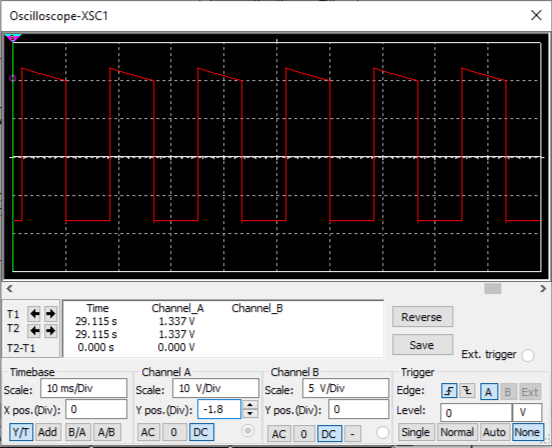
\includegraphics[width=0.975\textwidth]{images/simulacoes/osciloscopio_circuito06.png}
        }}
    \caption{Osciloscópio: Circuito retificador de onda completa B}
    \vspace{-0.3cm}
    \label{fig:OsciloscopioCircuito06}
\end{figure}

Através da imagem \ref{fig:OsciloscopioCircuito06}, podemos concluir que a entrada primária, que é representada pela linha verde, possui aproximadamente 311V, e a linha azul que representa a entrada secundária, possui aproximadamente 62.2V. Essa tensão é apresentada graficamente como sendo 30.631, pois a entrada secundária de 62.2 é dividida entre os dois diodos, sendo aproximadamente 31.1 para cada. A tensão de saída é a tensão sobre o resistor, e o sinal de saída tem o dobro da frequência.

Com a tabela \ref{tab:Comparacao6Circuito} podemos comparar os resultados obtidos por simulação com os resultados obtidos por cálculo, na qual comprovam que os cálculos estavam corretos, com uma pequena diferença devido a aproximação.

\begin{quadro}[H]
    \centering
    \caption{Comparação entre os resultados obtidos por simulação e os resultados obtidos por cálculo do circuito A}
    \begin{tabular}{|C{0.19\textwidth}|C{0.18\textwidth}|C{0.18\textwidth}|C{0.18\textwidth}|C{0.18\textwidth}|}
        \hline
        \rowcolor[HTML]{C0C0C0}
        \textbf{Modelo\textbackslash{}Variáveis} & \textbf{Tensão Pico primária} & \textbf{Tensão Pico secundária} & \textbf{Tensão pico de saída} & \textbf{Tensão pico média}\\
        \hline
        Calculado & 311V & 62.2V & 30.4V & 19.35V \\
        \hline
        Simulado & 306.444V & 61.262V & 29.751V & 18.97V \\
        \hline
    \end{tabular}
    \vspace{-0.6cm}
    \label{tab:Comparacao6Circuito}
\end{quadro} \clearpage
\chapter{CONCLUSÃO}

Através deste relatório, o autor conseguiu entender o funcionamento de um diodo de forma básica, onde o mesmo tem o funcionamento de chave fechada ou aberta, mas através disso, foi possível entender, sua composição, além de entender o comportamento seu comportamento e sua aplicação em circuitos. Sendo assim, o diodo é um componente eletrônico que permite a passagem da corrente em somente um sentido.

Pode-se afirmar que o diodo possui diversas aplicações, e uma delas é atuar como um retificador, convertendo tensão alternada em continua. Porém, deve-se atentar que um diodo possui energia dissipada em formato de calor, e por isso, deve-se ter cuidado com a quantidade de corrente que passa por ele, pois pode causar um superaquecimento, e consequentemente, danificar o componente. Além disso, o diodo possui uma aplicação em circuitos de proteção, onde o mesmo pode ser utilizado para proteger circuitos de tensões altas, como por exemplo, em circuitos de proteção de baterias, onde o mesmo pode ser utilizado para proteger o circuito de uma bateria de um curto-circuito, ou até mesmo, de uma descarga excessiva. \clearpage

\postextual

\bibliography{refs}

\end{document}
